\section{Greedy Algorithm}
\subsection*{Homework++ and Partition}
\textbf{Definition:}
Given some homework with start time, end time and duration of time. Give out whether we have a feasible solution to finish all the homework.
If greedy algorithm cannot promise a feasible solution, then no solution occurs.
different end time? do ddl sooner first.
different start time? do start time sooner first/ or arrange 
different release time/ deadline/size?Judge whether a solution exists(no need to find it)

Indeed, by Complexity Theory (), the problem is NP-hard. 
Consider a deliberately designed example: In \ref{fig:case_a}, we only have two types of work. For type one, 
However, either by choosing bigger or smaller size doesn't guarantee a feasible solution.
We claim that Partition problem is NP: Partition the set into two parts, whose sum are equal.
Given an input $a_1,\ldots,a_n$,let $w=\sum_{i=1}^n a_i$.
n normal homework starts at 0 and ends at $w+1$.
Special homework has release time $w/2$ , deadline $w/2+1$ and size 1.
Therefore, a special case for Homework++ is a Partition Problem.

NP: difficult to find answer, but easy to verify.

\subsection{Prim and Kruskal: Minimum spanning tree}
\textbf{Definition:}
A Minimum spanning tree (MSP) is the spanning tree( a tree that connects to all the edges) with the minumum total weight.

\textbf{Property:}
Shift edge operation on a cycle doesn't affect connectivity.

\subsubsection{Prim's Algorithm}
\textbf{Prim's Algorithm:} 

Adding the edge out of the previous Tree $T_i$ with the minimum weight to form $T_{i+1}$.\\
\textbf{Correctness of algorithm:}

The key idea for Prim is to guarantee that the tree with $n$ edges $T_n$ is a subset of \textbf{global} MST $T$. 
In inductive step, if $T_{i}$ is part of $T$, then we can construct $T_{i+1}$, s.t. $T_{i+1}\in T$.
Consider the first edge $e$ out of $T_{i}$, if $e=(u,v) \notin T$, then adding $e$ to $T$ constructs a cycle $C$. 
Since $e$ rather than $e' \in C, e' \notin T_{i}, e' \in T$, $w(e')\geq w(e)$. Since $T$ is the smallest spanning tree, $T-w(e')+w(e)\geq T$, $w(e)\geq w(e')$, therefore, $w(e)=w(e')$. Therefore, by shifting the two edges guarantees $T_{i+1}$ is a MST component of $T$.\\
\textbf{Time complexity:} $O(|E|\log(|E|))$.\\





\subsubsection{Kruskal's Algorithm}
\textbf{Kruskal's algorithm:} 

Similar to Prim's algorithm, it adds the smallest weighted edge that doesn't form a cycle with $T_{i-1}$ to form $T_i$.\\
\textbf{Correctness of Kruskal:} 

Similar to correctness of Prim, but the shift edge operation happens between components in a forest.\\
\textbf{Time complxity:}

$O(|E|\log(|E|))$ for sorting edges, and $|E|$ iterations of finding the representative element. A faster data structure is by \textbf{unified set}.\\
\subsubsection{unified set} 
store groups by their representative element (the children are represented by the root vertice of their tree).
\begin{enumerate}[-]
    \item Find: return the representative element in a group.($2|E|$)
    \item Union: Merge two groups.($|V|-1$)
\end{enumerate}
\begin{algorithm}
    \caption{Kruskal's Algorithm}
    Sort the edge set E to ascending order.\\
    X=\{\}\\
    For each $u\in V$, makeset($u$).\# $|V|$ create group\\
    For each $(u,v) \in E$ in ascending order\\
    \If {$find(u) \neq find(v)$}{
        Add edge $(u,v)$ to X\\
        % \union(u,v)\\
    }
    \SetKwFunction{union}{union}
    \SetKwFunction{makeset}{mk}
    \SetKwFunction{find}{find}
    \SetKwProg{Fn}{Function}{:}{}
    \Fn{\union{u,v}}{

    }
    \Fn{\find{$x$}}{
        \While{$x \neq pre(x)$}{

        }
    }
    \Fn{\union{$v$}}{

    }
\end{algorithm}

\begin{enumerate}
    \item \textbf{Path Compression:} Set the parent of the nodes checked to representative element.
    \item \textbf{time compexty analysis by Amortized Cost:}
\end{enumerate}


\textbf{check cycle:}

\subsection{Set Coverage}
\textbf{definition:}

\textbf{set Cover:} 
Find a sub-collection $S \subseteq T$ with minimum $|S|$ such that $\bigcup_{A_i\in S}A_i=U$.

\textbf{max k coverage:} 
Given $k \in N$, find a sub-collection $S\supseteq T$ with $|S|\leq k$ that maximizes element number it covers. Denote $f(S)=|\bigcup _{A_i\in S}A_i|$.

Also viewed in bipartite graph, with the left set be set index, and the right set be the node index. Edges across two sets means that $node \in set$.
\begin{remark}
\textbf{Approximation Algorithm:}

For maximize problem, algorithm $\mathcal{A} $ is called $\alpha$-approximation algorithm if $\frac{\mathcal{A}(I)}{OPTIM(I)}\geq \alpha$. Normally, time complexity should be polynomial.
\end{remark}

\begin{figure}
	\centering
    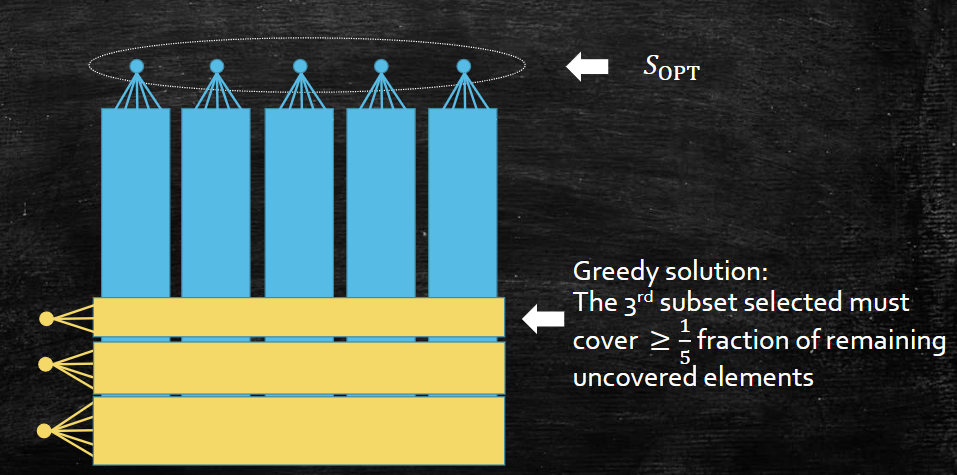
\includegraphics[width=0.8\linewidth]{Notes/fig/setcover.png}
    \caption{Directed Graph}
    \label{fig:setcover}
\end{figure}

We deliberately construct the worst case:
$|W_1|\geq \frac{1}{5}\text{biggest of remaining sets}$.
$W_1\cup W_2=1/5+1/5(1-1/5)=1-(1-1/5)^2$.
$f(S)\geq (1-(1-1/k)^k)$
\begin{lemma}
After choosing $l$ sets, $f(S)\geq (1-(1-1/k)^l)f(S^*)$, where $f(S^*)$ is the optim. sol. 
\end{lemma}
\begin{prf}
    Denote $S=\{A_1,\ldots A_m\}$, $S_t=\{A_1,\ldots A_t\}$, optim solution $S^*=\{O_1,\ldots, O_n\}$

    For base step, $l=1$,by greedy nature, $f(S1={A1})\geq f({O_i})$ for all $O_i$.
    Thus $f(S_1)\geq \frac{1}{k}\sum_{O_i \in S^*}f({O_i})=(1-(1-\frac{1}{k})^1)f(S^*)$ This implies when calculating the sum, union elements are calculated more than once.
    Also, the size of the first chosen set is larger than the average size of the optimal solution.
    Denote $\Delta(O_t|S_t)=f(S_t\cup {O_i})-f(S_t)$.

    $\Delta(A_{t+1}|S_t)\geq1/k\Delta(S^*|S_t)\geq \frac{1}{k}\Delta(S^*|S_t)$.
    For inductive step, suppose $f(S_t)\geq (1-(1-1/k)^t)f(S^*) $ 
    $f(S_{t+1})-f(S_t)\geq \frac{1}{k}(f(S^*\cup S_t)-f(S_t))\geq \frac{1}{k}(f(S^*)-f(S_t))$.
    $f(S_{t+1})\geq \frac{1}{k}f(S^*) + (1-\frac{1}{k})f(S_t)
    \geq \frac{1}{k}f(S^*) + (1-\frac{1}{k})(1-(1-1/k)^t)f(S^*)=((1-(1-1/k)^{t+1})f(S^*))$.
\end{prf}
For max-k-coverage, we at most choose $k$ sets.
$\lim_{k\rightarrow \infty}(1-(1-1/k)^l) =1-1/e$.
For set cover problem, it is a $ln n$ approximation.
$f(S)\geq 1-(1-1/k)^{k\cdot ln n}>(1-1/e^{ln n})=n-1$ Therefore, $f(S)=n$.

\subsection{Huffman Coding}
\begin{enumerate}
    \item prefix-free coding: each encoding is not a prefix of other encodings, i.e.,no vertice is an ancestor of others.
    \item optim prefix code(with minimum avg\_len):$avg\_len=\sum w(\sigma)\cdot len(\sigma)$, where $w$ is the frequency and $len$ is the length of the encoding.
    \item Huffman Tree is constructed by replacing two vertice with minimum $w$ with a new parent vertice whose weight is their weight sum repeatedly.
    \item The correctness is guaranteed. An intuitive way is the more frequent an encoding appears, the shorter the encoding is.
    Denote $T$ as the Huffman Tree, and $T'$ the tree that switched $u,v$, where $len(u)<len(v)$, $w(u)>w(v)$.
    avg\_len(T)-avg\_len(T')=$w(u)\cdot len(u)+w(v)\cdot len(v)-w(v)len(u)-w(u)len(v)=(w(u)-w(v))(len(u)-len(v)) <0$.

    Next, we'll guarantee that every next step is optim, i.e. $T_{i-1}$ is part of $T$.
    For base step,...
    For inductive step: If we merge $A$ and $B$ in $T$. If $A$ is paired with $C$ in $T^*$, then $w(C)>w(A)$ ,$w(B)\leq w(C)$. If $w(B)=w(C)$, changing B and C preserves avg\_len.
    If $w(B)\leq w(C)$, if $len(B)<len(C)$, contradiction! If $len(B)>len(C)$, swapping B and C also preserves avg\_len. If $len(B)>len(C)$, D is not processed, $w(D)\geq max(w(A),w(B))$

    Another intepretation is by sorting inequality, namely, the sum of $\sum ordered\_sequence \leq \sum random\_sequence \leq \sum inversed\_sequence$.
    \item \textbf{time complexity analysis} By using binary-heap, every time we conduct pop twice to obtain the top two min vertice and a push to add the new parent vertice in the tree.
\end{enumerate}

\subsubsection{K-Centers}
Find a set of k centers, $S=\{s_1,\ldots ,s_k\} \subseteq V$, $|S|=k$ that minimizes $f(S)=\max_{v \in V} \min_{s \in S} (s,v)$ which means the maximim distance of any vertex $v \in V$ to its closest center $s\in S$.
Note: k-center(2), k-means(9), k-median(5) are all np-hard, but have relatively good approximation algorithms.
\begin{remark}
    (V,d) is a matrix space if:
    \begin{enumerate}
        \item d(v1,v2)=0 iff v1=v2
        \item d(v1,v2)=d(v2,v1)
        \item $d(v1,v3)+d(v3,v2)\geq d(v1,v2)$
    \end{enumerate}
    e.g., G=(V,E,$w>0$)
\end{remark}
\textbf{Algorithm:} Iteratively pick the center farthest to the existing centers. Pick the first by random. by Dijkstra for weighted graph and BFS for unweighted.\\
Note: Intuitively, we want to choose the vertex with largest degree. However, this guarantees that more vertice are closer to center,
but isn't align with our objective of minimizing the dist(furthest vertice).\\
\begin{algorithm}
    \KwIn{metric space (V,d)}
    \KwOut{A set of k centers, $S$ that minimizes $f(S)=\max_{v \in V} \min_{s \in S} (s,v)$}
\end{algorithm}
\textbf{analysis of approximation algorithm}
% figure to be added
The algorithm is 2-approximation.
Denote $OPT=\max \min d(o_1,v)$. $A=\{a_1,\ldots a_k\}$ for algorithm result, $X_i=\{v_1,\ldots v_i\}$ as the set of vertice closest to $o_i$, optim solution $O=\{o_1,\ldots, o_k\}$

Case 1:Suppose $A\cap X_i \neq \emptyset$ Then each $X_i$ contains a center. As the biggest length between two vertice in $X_i$ is smaller than 2optim.

Case 2:Suppose $\exists A \cap X_i =\emptyset$. Suppose we choose $a_j$ and $a_r\in X_i$. Let $a_r$ be the second center chosen in $X_i$.
By greedy choice, $ALG=d(A,a_r)\leq d(a_j,a_r)$ before $a_r$ was chosen. Additionally, $d(a_j,a_r)\leq d(a_j,o_i)+d(a_r,o_i)\leq 2OPT$.


Also, it is the best algorithm.
\textbf{dominated set} a dominating set is a
subset of vertices $S$ such that, for any $v \in V \ S$, there is a
vertex $u \in S$ that is adjacent to $v$.
A dominated set problem(output whether a dominated set exists) is an NP problem.
If $\exists$ a polynomial time $(2-\epsilon)$-approximation algorithm $\mathcal{A} $ for K-center. Denote the algorithm with slight modification running on $(G,k)$ to output dominated set result as If $\mathcal{A'}$.
If $\mathcal{A'}(G,k)=Yes$, $OPT\leq 1$. If $\mathcal{A'}(G,k)=No$, $ANS\geq 2$,$OPT \geq 2/(2-\epsilon)$.
Therefore, $G$ has a dominated set of size k iff K-center solution of $(G,k)$ output by $A$ has cost 1.
Also called gap(amplifying)-reduction.

\textbf{local search on k-center}

Two ways to solve NPH problem, either by hyristic algorithm (with no approximation lower bound or guarantee of optimal solution) or approximation, restrictions on the input,

\subsubsection{local search: max-cut}
\begin{enumerate}
    \item \textbf{Time Complexity} checking whether to update takes $O(|E|)$, every update you earns at least an edge, so it takes $O(|E|)$ rounds. The total algorithm is $O(|E|^2)$, polynomial!
    \item \textbf{Approximation} When the algorithm terminates, $\forall u$, at least 0.5deg(u) edges are in the cut, which leads to a 0.5-approximation.
     \[c(A,B)\geq \frac{1}{2}\sum_{u\in V}\frac{1}{2}deg(u)=\frac{1}{2}|E|\]
    \item better approximation algorithm: 0.878-approximation(semi-definite programming)
    % \item https://zhuanlan.zhihu.com/p/69126787
\end{enumerate}

palindrome: a string that reads the same backward as forward, e.g., madam, racecar, abba, etc.
